
\documentclass[11pt]{article}
\usepackage{amsmath}
\usepackage{siunitx}
\usepackage{graphicx, float}
\usepackage[OT1]{fontenc}
\renewcommand*\familydefault{\sfdefault}

\title{Measuring Modes on Strings: Part 1}
\author{Alex Booth}

\begin{document}
    \maketitle

    \section{Introduction}
        This report details an investigation into the phenomena observed on a vibrating string.
        Several experiments took place, using a guitar, as guitars feature strings under tension that can freely vibrate.
        The frequency and amplitude of vibrations can be easily and precisely adjusted on a well-intonated guitar by fretting the strings along the fingerboard.
        Results are tabulated and plotted on graphs using MATLAB. 
    
    \section{Theory}
        A string vibrates with a fundamental, or in music theory tonic, frequency.
        This fundamental frequency is related to the length $L$ of a vibrating string:
        \begin{equation}
            f_1 = \frac{c}{2 L}
        \end{equation}
        The mass of a string and its length can be used to find a mass per unit length $M$.
        This mass per unit length can then be formulated with it's tension $T$ to find the speed of a transverse wave on a string:
        \begin{equation}\label{speed}
            c = \sqrt{\frac{T}{M}}
        \end{equation}
        Equation \ref{speed} allows us to formulate:
        \begin{equation}\label{fund}
            f_1 = \frac{\sqrt{\frac{T}{M}}}{2 L}
        \end{equation}
        If the ends of a string under tension are fixed, the fundamental frequency will have a wavelength equal to half the string's length.
        The frequencies of higher harmonics of the fundamental frequency are integer multiples of the fundamental frequency:
        \begin{equation}\label{harm}
            f_n = \frac{c}{2 L} n
        \end{equation}

    \section{Experiment One}
        \subsection{Methodology and Results}
            In experiment one, the relationship between resonant frequency and string length were investigated.
            Preliminary measurements of mass and length were taken in order to find a mass per unit length $M = 0.012618\si{\kilogram\per\meter}$.
            Then the low E string was played in an open position, thus at it's maximum string length and at a frequency of $83\si{\hertz}$.
            Using equation \ref{harm} the higher harmonics $n = 1, 2 ,3 ...$ are predicted for the vibrating open E string.
            The sound of the vibrating string was captured using a microphone and passed into a Simulink frequency spectrum analyser.
            From this spectrum analyser the frequencies of the fundamental tone and it's higher harmonics could be ascertained.
            However, not every frequency in the harmonic series had a sufficient amplitude to be declared a peak by the Simulink spectrometer, meaning that the recorded harmonic series will have gaps compared to the array of predicted harmonic frequencies.
            Rearranging equation \ref{harm} allowed a wave speed $c_n$ to be found for each harmonic number, for both the predicted and recorded harmonics.
            To compare the error between the predicted and observed harmonic wave speeds, a mean wave speed was taken for the observed values.
            The difference between this mean wave speed $c$ and each predicted harmonic wave speed $c_n$ was then taken.
            These differences were then summed and divided by the number of harmonics to give a mean difference and thus average error:
            \begin{equation}
                \Delta c = \frac{1}{N}\sum_{n=1}^{N} | c_n - c |
            \end{equation}
            The array of predicted wave speeds for harmonic numbers up to harmonic number $n=6$ are tabulated:
            \begin{table}[H]
                \centering
                \begin{tabular}{c | l l l l l l}
                    \hline
                    $n$ & 1 & 2 & 3 & 4 & 5 & 6 \\
                    \hline
                    $c(\si{\meter\per\second})$ & 102.7 & 205.41 & 308.12 & 410.83 & 513.54 & 616.24 \\
                    \hline
                \end{tabular}
                \caption{Predicted wave speeds for each harmonic}
            \end{table}
            The average error $\Delta c$ was calculated: $\Delta c = 30.812$.
            \newpage
            Next, the guitar string was plucked whilst fretted on the fingerboard.
            The fundamental frequency for the fretted note (A - the 5\textsuperscript{th} fret on the E string) was predicted to be $f=110\si{\hertz}$ using equations \ref{speed} and \ref{harm}.
            The recorded frequency was found to be $f=112\si{\hertz}$.
            The string was fretted at a series of frets and the fundamental frequencies were tabulated:
            \begin{table}[H]
                \centering
                \begin{tabular}{c | l l l l}
                    \hline
                    Fret & 0 & 3 & 5 & 12 \\
                    \hline
                    Distance from bridge (\si{\meter}) & 0.645 & 0.534 & 0.477 & 0.318 \\
                    \hline
                    $f_1(\si{\hertz})$ & 81 & 97 & 113 & 167 \\
                    \hline
                \end{tabular}
                \caption{Fundamental frequencies of each fretted note}
            \end{table}
            Using equation \ref{fund}, an array of predicted values for fundamental frequency can be found and plotted against string length.
            The observed fundamental frequencies for each fretted note are also plotted on the same graph.
            \begin{figure}[H]
                \centering
                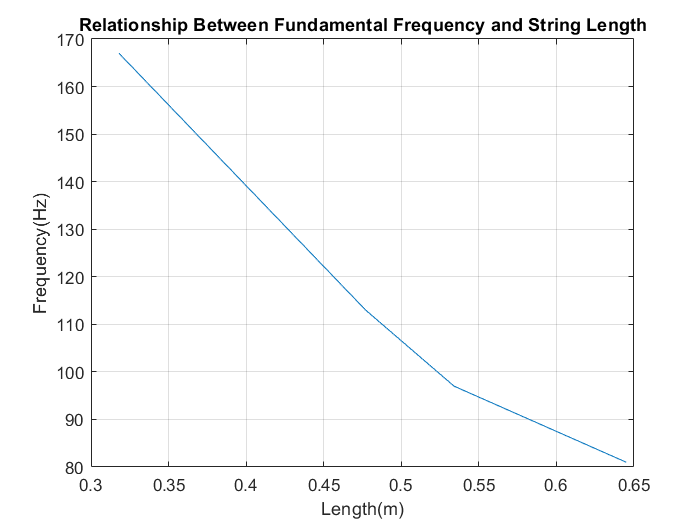
\includegraphics[scale=0.5]{resources/F1vsL.png}
            \end{figure}
        \subsection{Discussion of Results}
            Such a high error can be attributed to the missing harmonic frequencies from the observed series, and the frequency response of the microphone used to capture the sound "colouring" the signal.
    \section{Experiment 2}
            \subsection{Methodology and Results}
            Rearranging equation \ref{speed} allows us to find a value of Tension $T$ for the open string.
            The error of the results $\Delta T$ is depended on the error $\Delta c$. And thus the error $\Delta T$ was tabulated:
            \begin{table}[H]
                \centering
                \begin{tabular}{c | l l l l l l}
                    \hline
                    $n$ & 1 & 2 & 3 & 4 & 5 & 6 \\
                    \hline
                    $c(\si{\meter\per\second})$ & 102.7 & 205.41 & 308.12 & 410.83 & 513.54 & 616.24 \\
                    \hline
                \end{tabular}
                \caption{Error in string tension}
            \end{table}
            Next, the tension of the string was increased using the tuning peg.
            Adjusting the tension increased the fundamental frequency
    \section{Experiment 3}
        Plucking a string at different positions creates a different harmonic content in the radiated sound, even though the fundamental note remains the same.
        The guitar used in experiment one was plucked from various positions along the open E string.
        The frequency spectra of the radiated sound at each playing position were recorded. The closer to the ends under tension the string was plucked, the
        

\end{document}